\chapter{Methodology}

\section{Corrosion}

One of the main phenomenon that affect the long term behavior of RC structures is corrosion of the reinforcing steel. Two types of corrosion are possible:
\begin{itemize}
		\item Carbonation, 
		\item Chloride attack
\end{itemize}

The main source of corrosion in most RC structures is Chloride Attack and is the one that is assumed in the present study.

Corrosion of steel in concrete is an electrochemical process \cite{Mehta2014} this corrosion mat be generated in two ways:
\begin{itemize}
	\item Composition cells may be formed when to dissimilar metals are embedded in concrete or when significant variations exist in the surface characteristics of steel
	\item In the vicinity of steel concentration cells may be formed due to differences in the concentration of dissolved ions, such as alkalies and \textbf{chlorides}.
\end{itemize}

The corrosion process under chloride attack type of corrosion consists in first the protective film  on the reinforcing steel surface is destroyed, a process known as \textbf{depassivation}, then initiation of corrosion happens, the electrical resistivity and the oxygen content control corrosion. Figure \ref{fig:corr1} schematically show this process.

\begin{figure}[htbp]
\centering
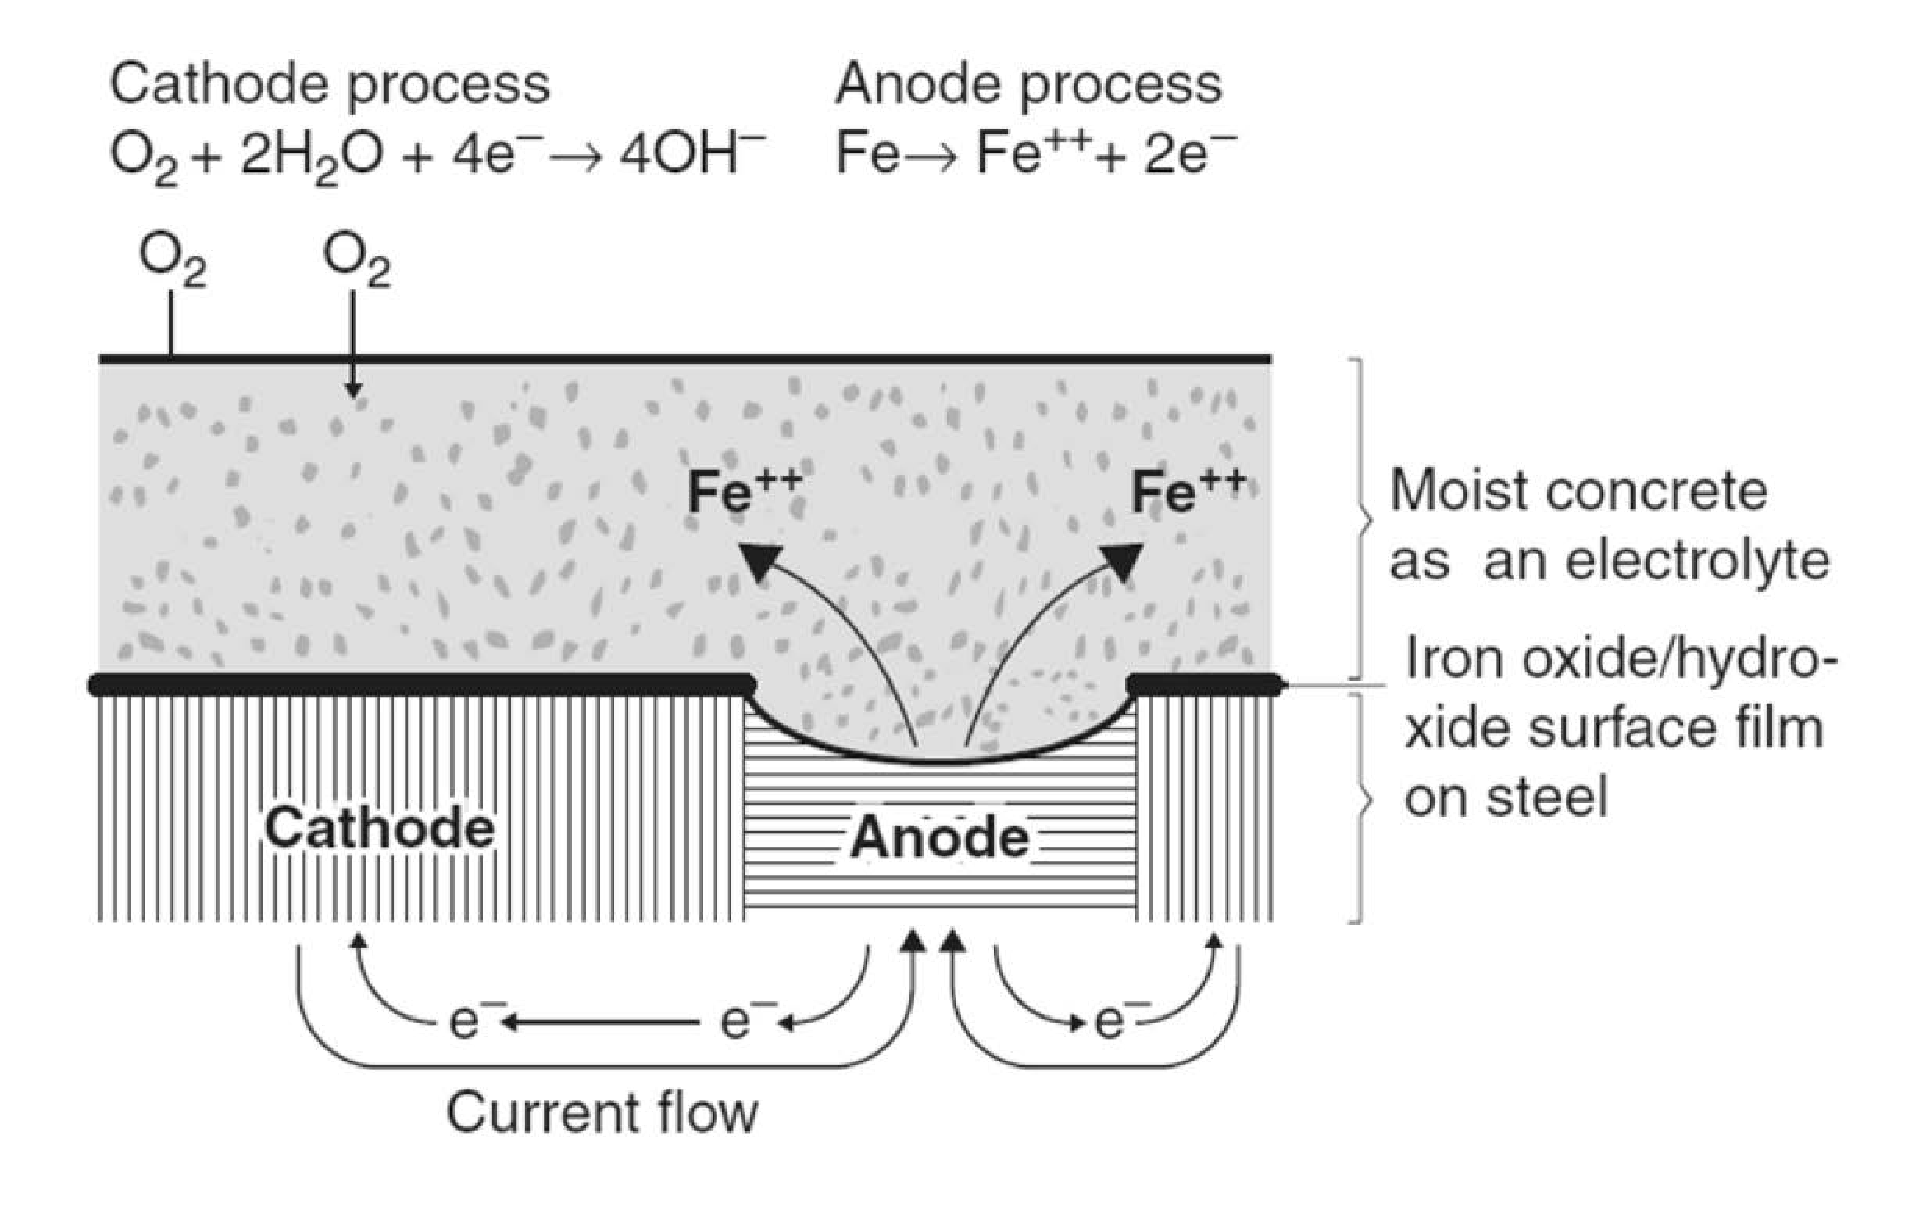
\includegraphics[width=0.9\textwidth]{Chapter-2/figs/Corrosion_Process}
\caption{Corrosion Process in Reinforcing Steel Bar \cite{Mehta2014}}
\label{fig:corr1}
\end{figure}


A literature review to characterize corrosion in reinforcing steel is presented such that corrosion can be modeled as a function of time, the corrosion process is an extensive field of research and to characterize it, therefore the different components of this subject are categorized as follows:

\begin{enumerate}
	\item Time to Initiation of Corrosion (Tcorr)
	\item Corrosion growth in reinforcing steel
	\item Mechanical Properties of Corroded Reinforcing Steel (fycorr, fucorr)
	\item Cyclic Test on Corroded RC Columns
	\item Flowchart of Corrosion Model Implemented
\end{enumerate}

 
\subsection{Time to Corrosion}

Time to corrosion refers to the corrosion initiation at which the passivation of steel is destroyed and reinforcement starts corroding actively.
\newline

\textbf{Christensen Model}
\newline

Christensen \cite{Thoft-Christensen} main goal was to generate a corrosion model that was general for all concrete elements, additionally the authors tried to generate a model that also included the appearance of cracks due to corrosion that would evetually grow and the spall the concrete. 

More specifically related to reinforcing steel corrosion they developed a model based on Fick's law of diffusion to model the rate of chloride penetration into concrete as a function of concrete cover and time. 

\begin{equation}
	\frac{\partial C(x,t)}{\partial t} = D_c \frac{\partial C(x,t)}{\partial x^2}
	\label{eq:one}
\end{equation}

After solving equation \ref{eq:one} the following expression results:
\begin{equation}
  T_{corr}=\frac{d^2}{4D_c} \left[erf^{-1}\left(\frac{C_{cr}-C_{0}}{C_1 -C_0}\right)\right]
  \label{eq:two}
\end{equation} 

$d$: Concrete cover

$D_0$: Diffusion coefficient

$C_{0}$: Equilibrium Chloride Concentration

$C_{cr}$: Critical chloride corrosion concentration
\newline

While this model provides a means to calculate the Time for initiation of corrosion as a function of Concrete Cover and Diffusion concentration, the estimation of the Diffusion concentration depends on several factors such as environment, curing and water to cement ratio it is not a reliable method to estimate the Time to Corrosion.
\newline

\textbf{Gosh \& Padgett Model}
\newline

Ghosh et al calculate time to corrosion based on Thoft-Christensen model, considering in-field corrosion related studies of existing bridge components in the United States exposed to deicing salts to obtain mean values of chlorides concentration and put them in a modified version of the Thoft-Christensen Model.

\begin{equation}
T_{corr}=\frac{x^2}{4 D_c} \left[erf^{-1} \left(\frac{C_0-C_cr}{C_0} \right) \right]^{-2}
  \label{eq.three}
\end{equation} 

$D_c$ 1.29 $frac{cm^2}{year}$ Diffusion Coefficient 

$C_0$ 0.10 Surface Chloride Concentration

$C_r$ 0.04 Critical Chloride Concentration
\newline

While this model provides mean values for the time of initiation of corrosion, it is limited to environments that are controlled by \textbf{dicing salts only}.
\newline

\textbf{Life 365}
\newline

Is a software developed by a consortium of companies of the cementitious materials industries and academic institutions. This software relies on the studies summarized above, mainly using the Thoft-Christensen model, but as opposed to assuming dicing environments only, this software uses a database of chlorides concentration for different location in the USA and Canada, which gives more accurate results depending on the location and environment in which the structure is located.

While this is a more robust model to obtain the initiation of corrosion since it considers the location and environment of the structure and it also has the ability to include other durability issues, it is difficult to implement in a batch run format since the program is in a closed format.
\newline

\textbf{Liu \& Weyers Model}
\newline

\begin{equation}
  T_{cr}=\frac{W_{crit}^2}{2k_p}
  \label{eq.four}
\end{equation} 

\begin{equation}
  W_{crit}=\rho_{rust} \left[ \pi \left[ \frac{C f'_t}{E_{ef}} \left( \frac{a^2+b^2}{a^2-b^2}+\nu_c \right)+d_o \right] D+ \frac{W_{st}}{\rho_{st}} \right]
  \label{eq.five}
\end{equation} 

\begin{equation}
  k_p=0.098 (\frac{1}{\alpha})\pi Di_{corr}
  \label{eq.six}
\end{equation} 

$W_{crit}$: Critical amount of corrosion needed to induce cracking.

$W_{st}$: Mass of corroded steel.

$\rho_{rust}$: Density of rust material.

$\rho_{st}$: Density of steel.

$f'_t$: Tensile strength of the concrete. 

$E_{ef}$: Effective elastic modulus of concrete $E_{ef}=\frac{E_c}{1+\phi_{crit}}$ 

$\phi_{crit}$ Creep coefficient of the concrete.

$D$: Diameter of bar.

$d_o$: Thickness of pore band around the steel/concrete interface.

$\nu_c$: Poisson's ratio of concrete.

$C$: Cover depth

$a=\frac{D+2d_o}{2}$

$b=C+\frac{D+2d_o}{2}$

\subsection{Rate of corrosion}

\textbf{Vu et al. Model }
\newline

To estimate the loss of steel cross section due to corrosion a time dependent corrosion rate model was developed by \cite{Vu2000}, this model implies that corrosion diminishes with time since as corrosion accumulates with time around the steel, it precludes uncorroded steel to react with the environment. The model is shown in \eref{eq.five}.

\begin{equation}
  i_{corr}=\frac{37.5(1-w/c)}{d_c}
  \label{eq.eight}
\end{equation} 

$w/c$: Water Cement ratio
$d_c$: Cover depth

In \fref{fig:hist1} the behavior of this model for different values of $w/c$ ratios is shown. It can be seen that at larger values of cover depth the rate of corrosion decreases rapidly and as the water cement ratio increases the rate of corrosion decreases.
%
\begin{figure}[htbp]
\centering
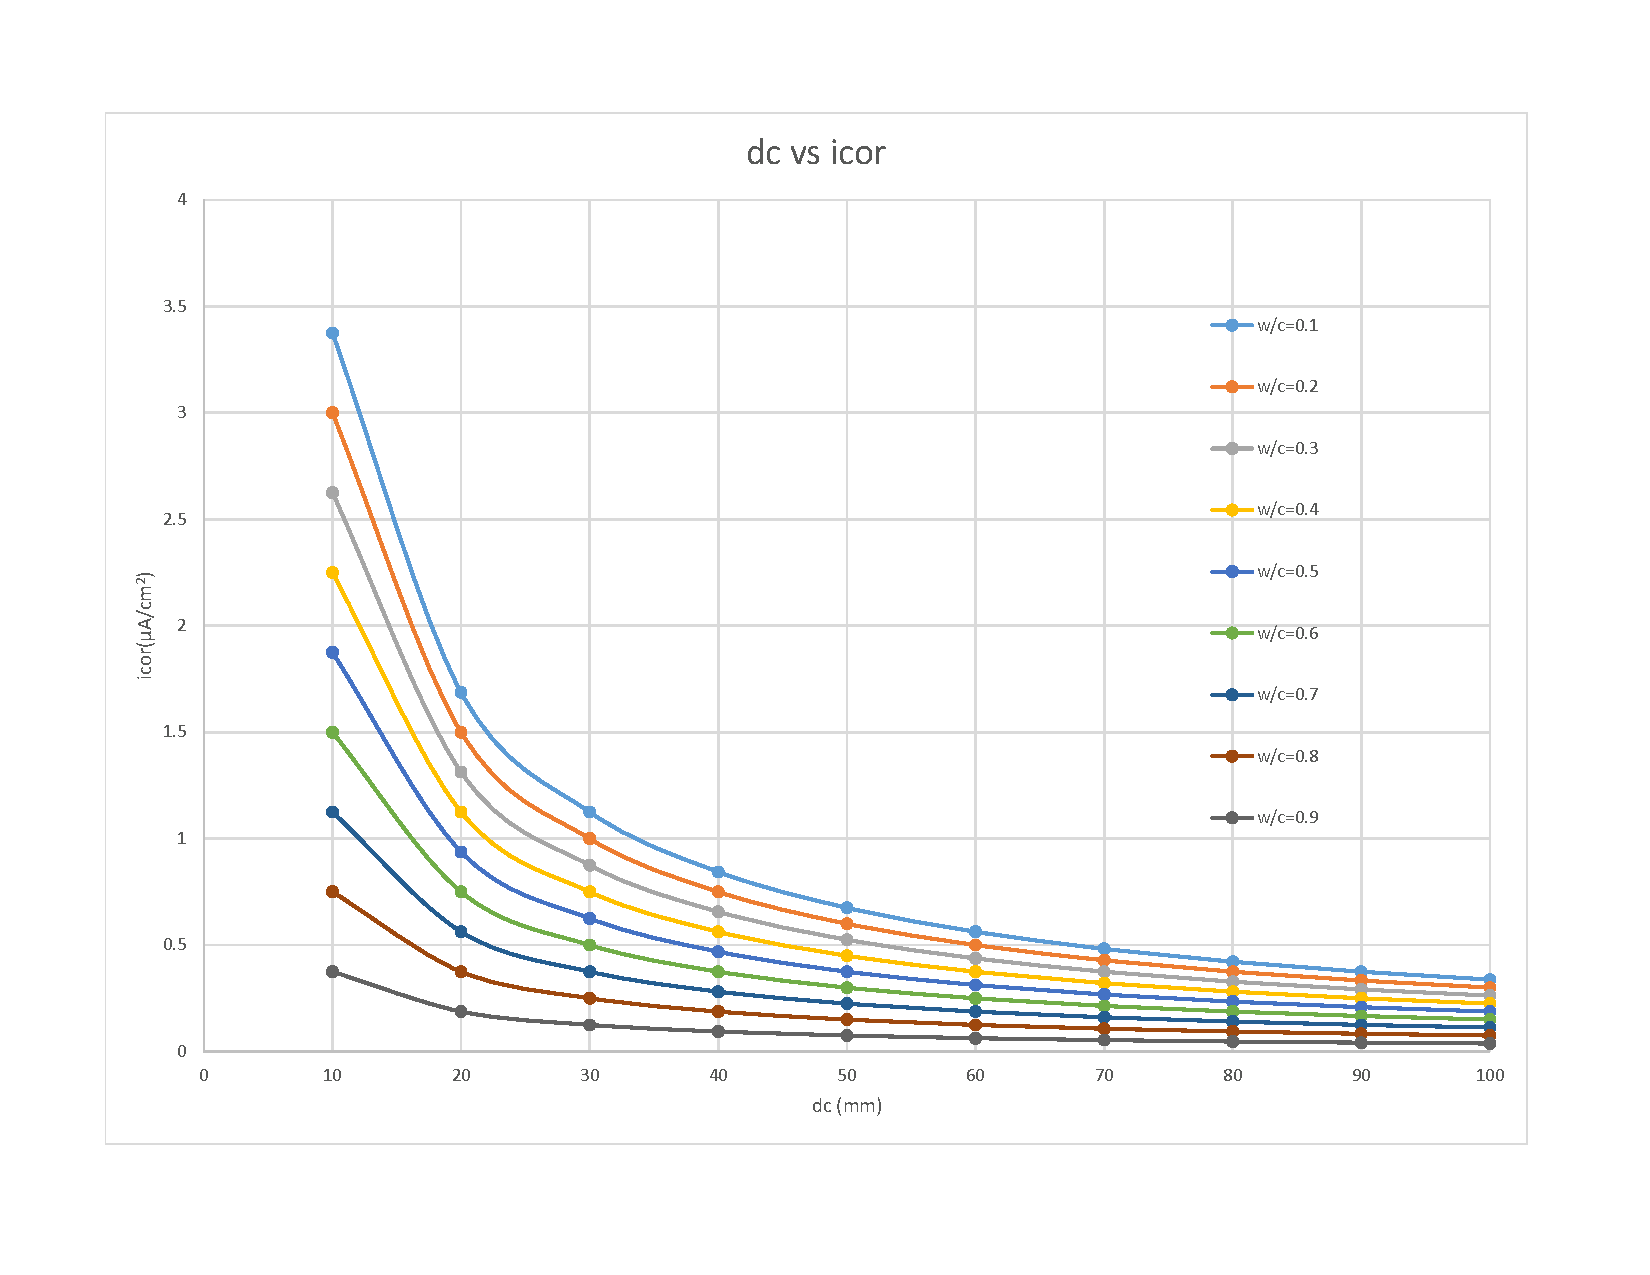
\includegraphics[width=0.7\textwidth]{Chapter-1/figs/dcvsicor}
\caption{Concrete cover depth vs rate of corrosion}
\label{fig:hist1}
\end{figure}

From the Vu et al model the diamater degradation is calculated according to Choe et al as:

\begin{equation}
  d_{corr}=d_{bi}-\frac{1.0508(1-w/c)}{d_c} (t-t_{corr})^{0.71}
  \label{eq.nine}
\end{equation} 

$d_{bi}$: Is the initial diameter of the bar

The diameter is plotted in \fref{fig:hist2}.

\begin{figure}[htbp]
\centering
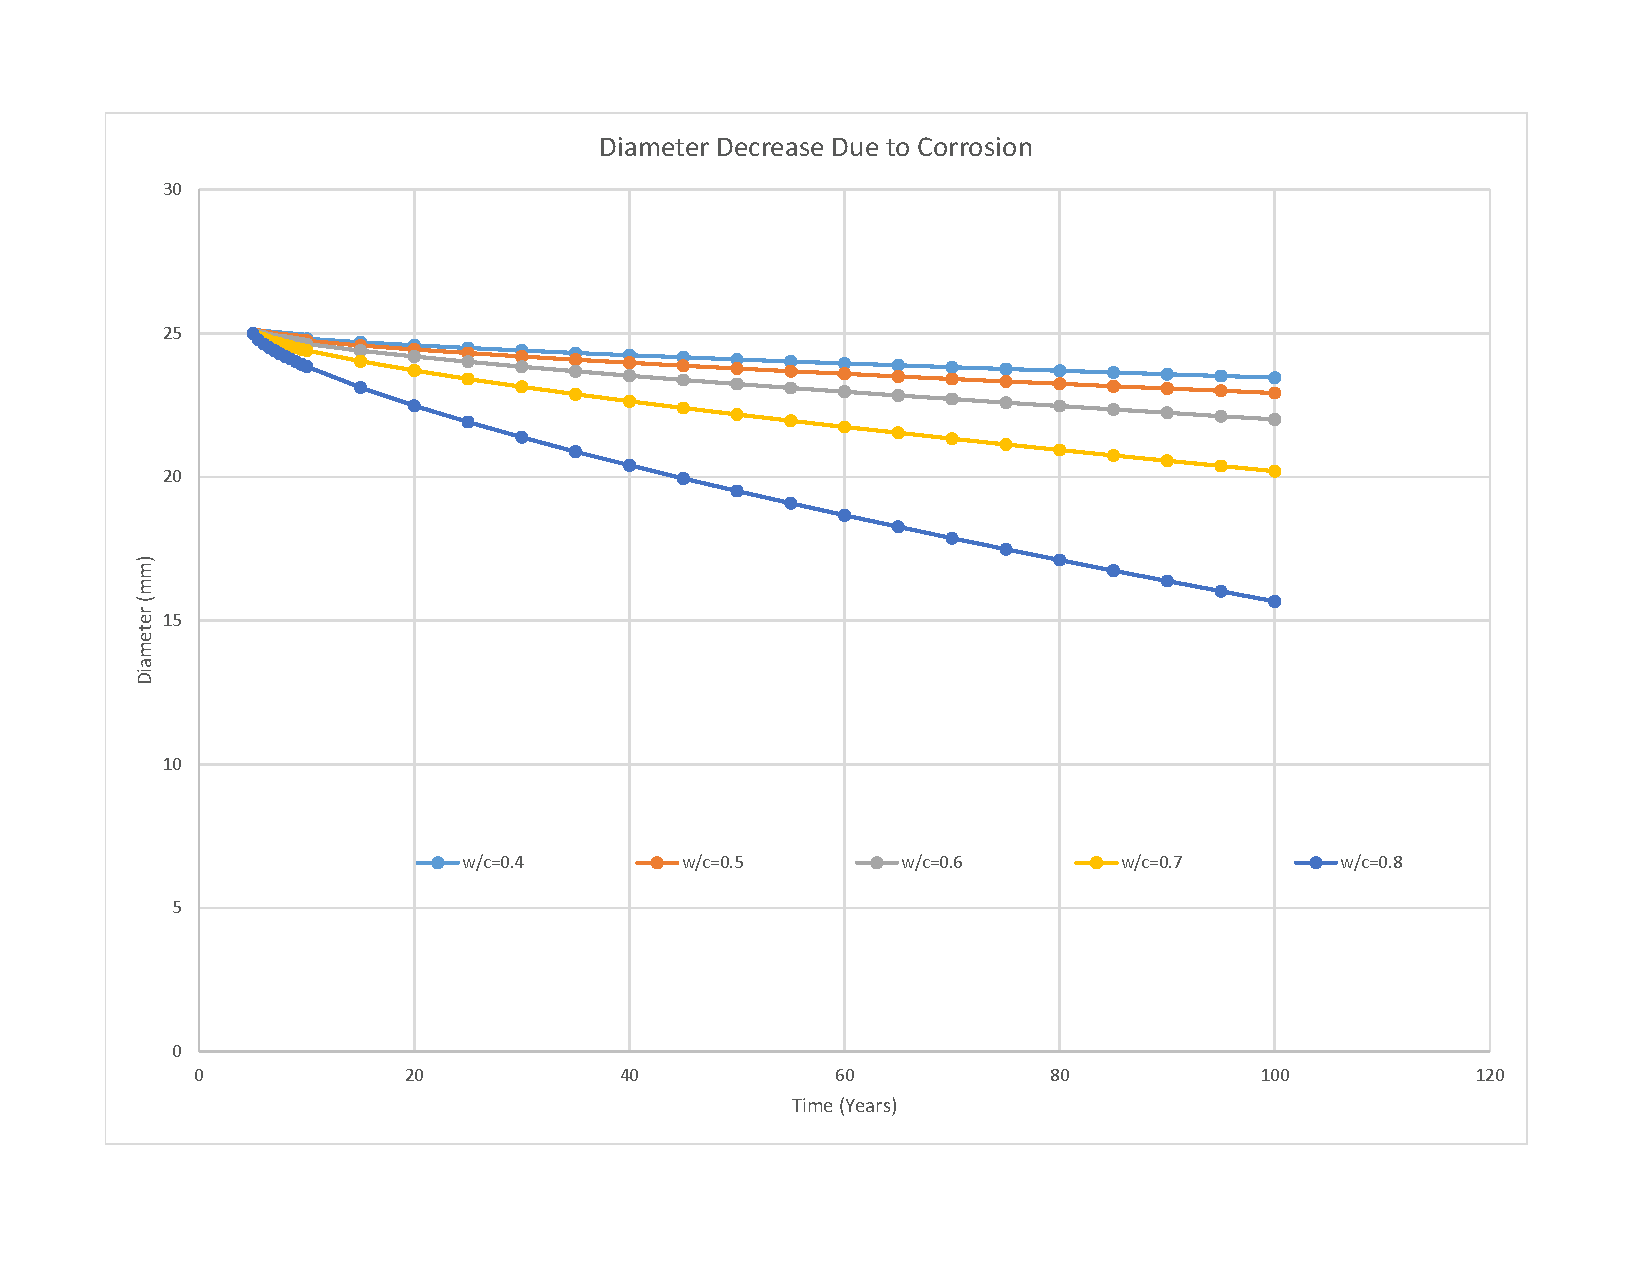
\includegraphics[width=0.7\textwidth]{Chapter-1/figs/DiameterDecrease}
\caption{Diameter decrease due to corrosion}
\label{fig:hist2}
\end{figure}

These values would correspond to a level of corrosion that varies from 7\% corrosion to 21\% of corrosion for w/c ratios that ranges from 0.4 to 0.6
The level of corrosion is calculated as:

\begin{equation}
  C=\frac{G_o-G}{g_ol_o} *100%
  \label{eq.ten}
\end{equation} 

Then the Corrosion level is plotted as a function of time in \fref{fig:hist3}

\begin{figure}[htbp]
\centering
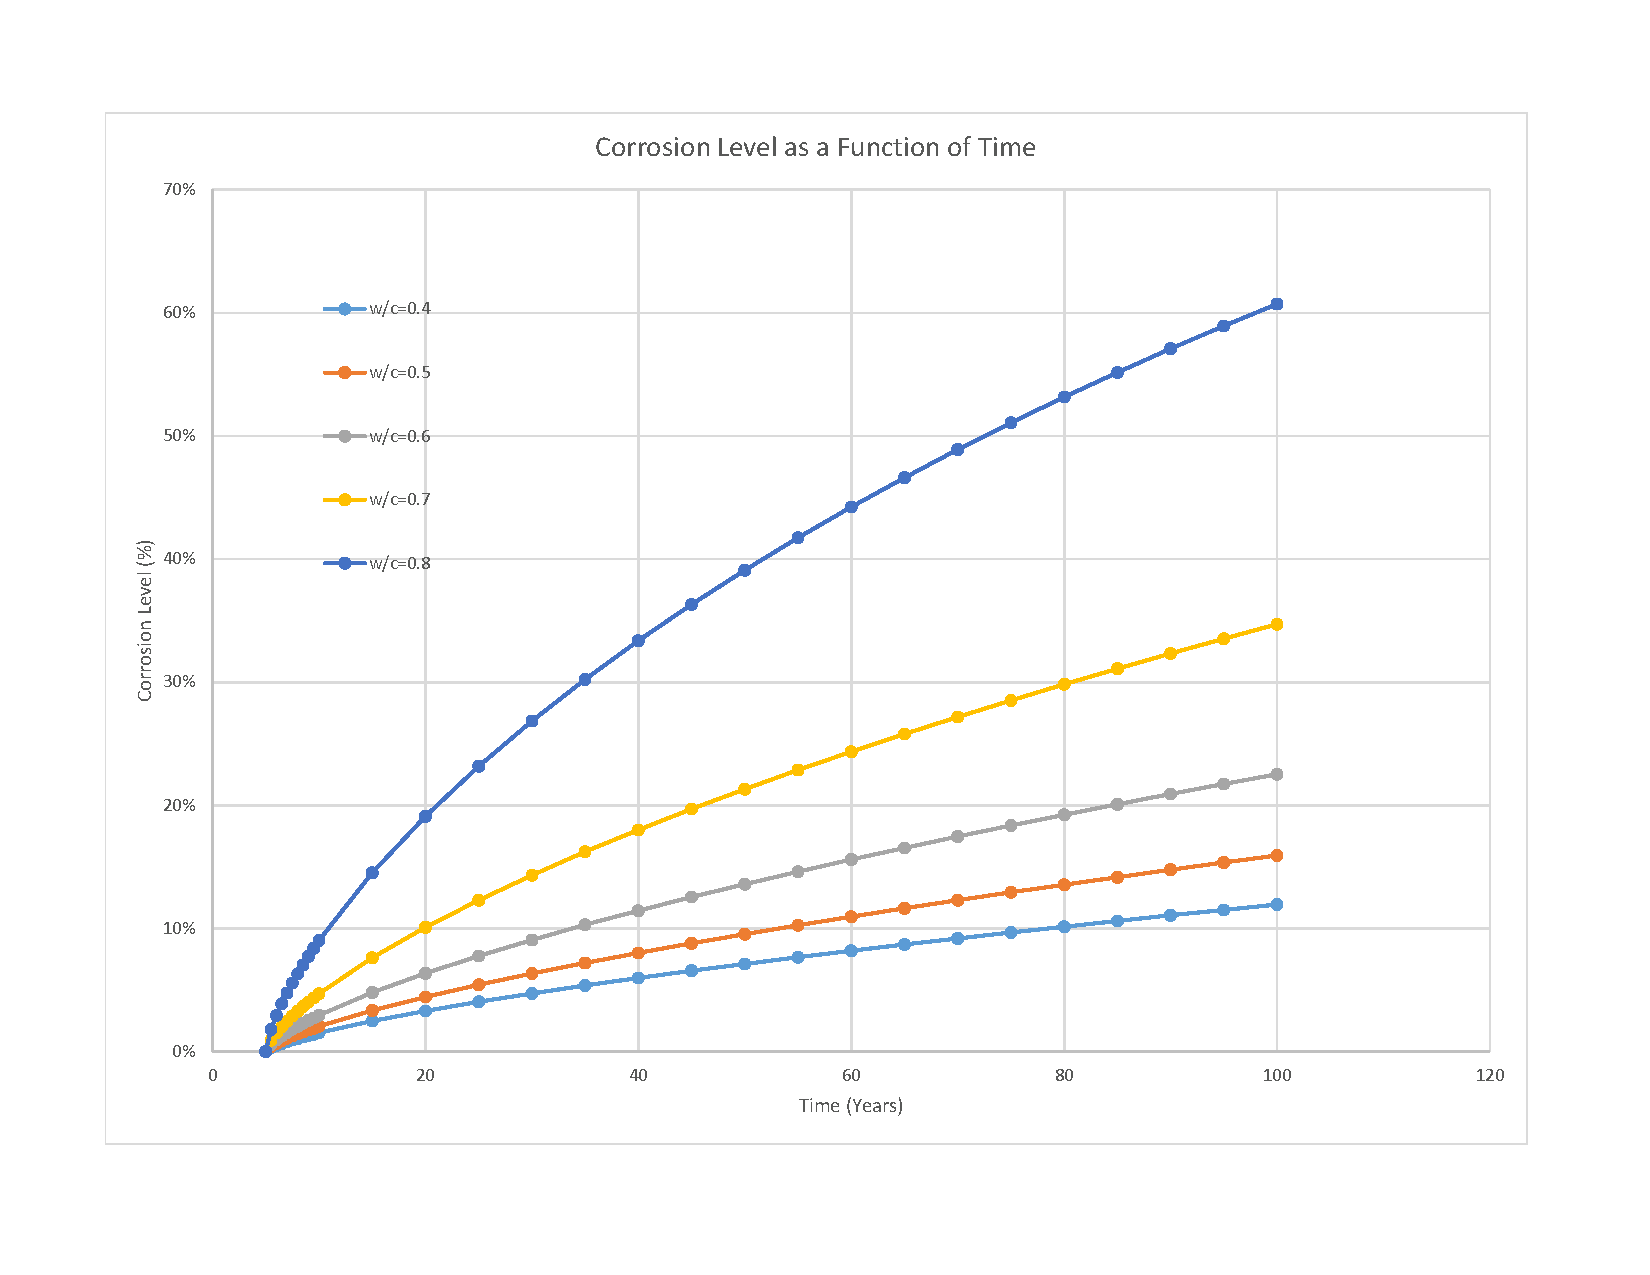
\includegraphics[width=0.7\textwidth]{Chapter-1/figs/CorrosionLevel}
\caption{Corrosion Level vs Time (years)}
\label{fig:hist3}
\end{figure}

\subsection{Corrosion modified properties of reinforcing steel bars}

In a study presented by Yuan et al \cite{Yuan2017a} it was shown from experimental results that the mechanical properties of steel for different levels of corrosion could be modified for analysis as follows:

\begin{equation}
  f_{y,C}=f_{yo}(1-0.021C)
  \label{eq.eleven}
\end{equation} 

\[
  f_{u,C}=f_{yo}(1.018-0.019C)
\]
\[
  \delta_{s,C}=\delta_{so}(1-0.021C)
\]
\[
  \varepsilon_{y,C}=\varepsilon_{yo}(1-0.021C)
\]

\:
\textbf{Choe et al. Model }
\:
Choe et al research is a seismic fragility estimates for RC columns subjected to corrosion, while the study is probabilistic in nature it defines the reduction in rebar cross section as:

\begin{equation}
	d_{b}(t)=d_{bi}-2\int_{T_{corr}}^{t} \lambda(t) dt
\end{equation}

Considering the model proposed by Vu et al the bar diameter degradation can be expressed as:

\begin{equation}
	d_{b}(t)=d_{bi}-\frac{1.508(1-\frac{w}{c})^-1.64}{d}(t-T_{corr})^0.71
\end{equation}

Where the diameter of the bar and the cover is in (mm).
Pros:
Easy way to calculate the reduction of bar diameter.
Cons:
The model carries out the assumptions made by Vu et al. concerning concentration of chlorides assumed and the diffusion assumed.

With this information, the corrosion level is calculated as:

\begin{equation}
	CL=\frac{d_{i}-d(t)}{d_{i}}
\end{equation}

\subsection{Corrosion modified properties of reinforcing steel bars}
\:
\textbf{Yuan et al. 2017}
\:
Yuan et al performed full-scale tests on columns with corroded longitudinal reinforcement, with which they proposed the following equation to characterize the effects of corrosion in reinforcing steel.

\begin{equation}
	f_{y}(t)=f_{y0}(1+0.021CL)
\end{equation}

While the equation showed, agreement with the test results that they performed it has not been corroborated by other researchers. In the current consensus, the model used is the one proposed by Du et al.


\textbf{Du et al. 2005}

Du et al investigated the effect of corrosion on the mechanical properties of steel using corrosion levels of 5%, 10%, 15% and 20%. Another variable that was researched was the type of rebar (smooth or ribbed), diameter of the rebar.
\begin{equation}
	f_{y}(t)=f_{y0}(1+0.021CL)
\end{equation}

\section{Steel Strain Aging}

\subsection{Metallurgical Process}

It is generally accepted that strain aging is due to the diffusion of carbon and/or nitrogen atoms in solution to dislocations that have been generated by plastic deformation. Initially, an atmosphere of carbon and nitrogen atoms is formed along the length of a dislocation, immobilizing it. Extended aging, however, results in sufficient carbon and nitrogen atoms for precipitates to form along the length of the dislocation.

These precipitates impede the motion of subsequent dislocations, and result in some hardening and loss in ductility. The extent of strain aging, which is a thermally activated process, depends primarily on aging time and temperature. In general, extended aging results in a saturation value above which further aging has no effect.

A second strengthening mechanism occurs when cold deformation (alone) is applied to steels. When dislocations break away for their pinning interstitial atoms and begin the movement causing slip they begin to intersect with each other. A complex series of interactions between the dislocations occurs, causing them to pin each other, decreasing their mobility. The decreased mobility also results in higher strength, lower ductility and lower toughness. As a result, cold deformed steels already have lowered ductility and toughness before any strain aging occurs and when heating follows cold deformation, the loss in ductility and toughness is greater. It is this combination of events that is the most damaging to the toughness of structural steels.

\subsection{Strain aging effects in structures}

Since it has already been established that strain aging is the process in which steel after being subjected to large strains develops an increased strength and reduced ductility with time and therefore important to include it in a time dependent analysis, considering the fact that plastic hinges will form in a ductile structure and the steel could reach high strains in this regions of the structure. Furthermore strain aging will cause an increased in the strength of the plastic hinge and as a consequence plastic hinges might be formed in regions of the structures that have not been designed for such demands. The effects of strain aging may also alter the transverse reinforcement due to both cold bending, making them susceptible to brittle failure.

According to \cite{Restrepo-Posada1994} most strain aging occurs in the first 37 days. Also \cite{Momtahan2009} studied strain aging effects with respect to time for different levels of pre-strains that ranged from $2\varepsilon_y - 10\varepsilon_y$ and for a time frame of 3 days to 50 days, from this study it was determined that a significant effect of strain aging took place from pre-strains $5\varepsilon_y$ and on. Strains higher than $15\varepsilon_y$ indicate a performance level in which substantial damage has been induced in the structure such that it is deemed unrepairable and therefore pre-strains higher that $15\varepsilon_y$ are unpractical and not studied by Montahan et al\cite{Momtahan2009}.
\\
\textbf{Momtahan et al Strain Aging Effects in Yield Strength of Steel}

Momtahan et al was able to correlate the increase in yield strength as a function of time and the pre-strain in reinforcing steel bars. The proposed equations are shown below:

\begin{figure}[htbp]
\centering
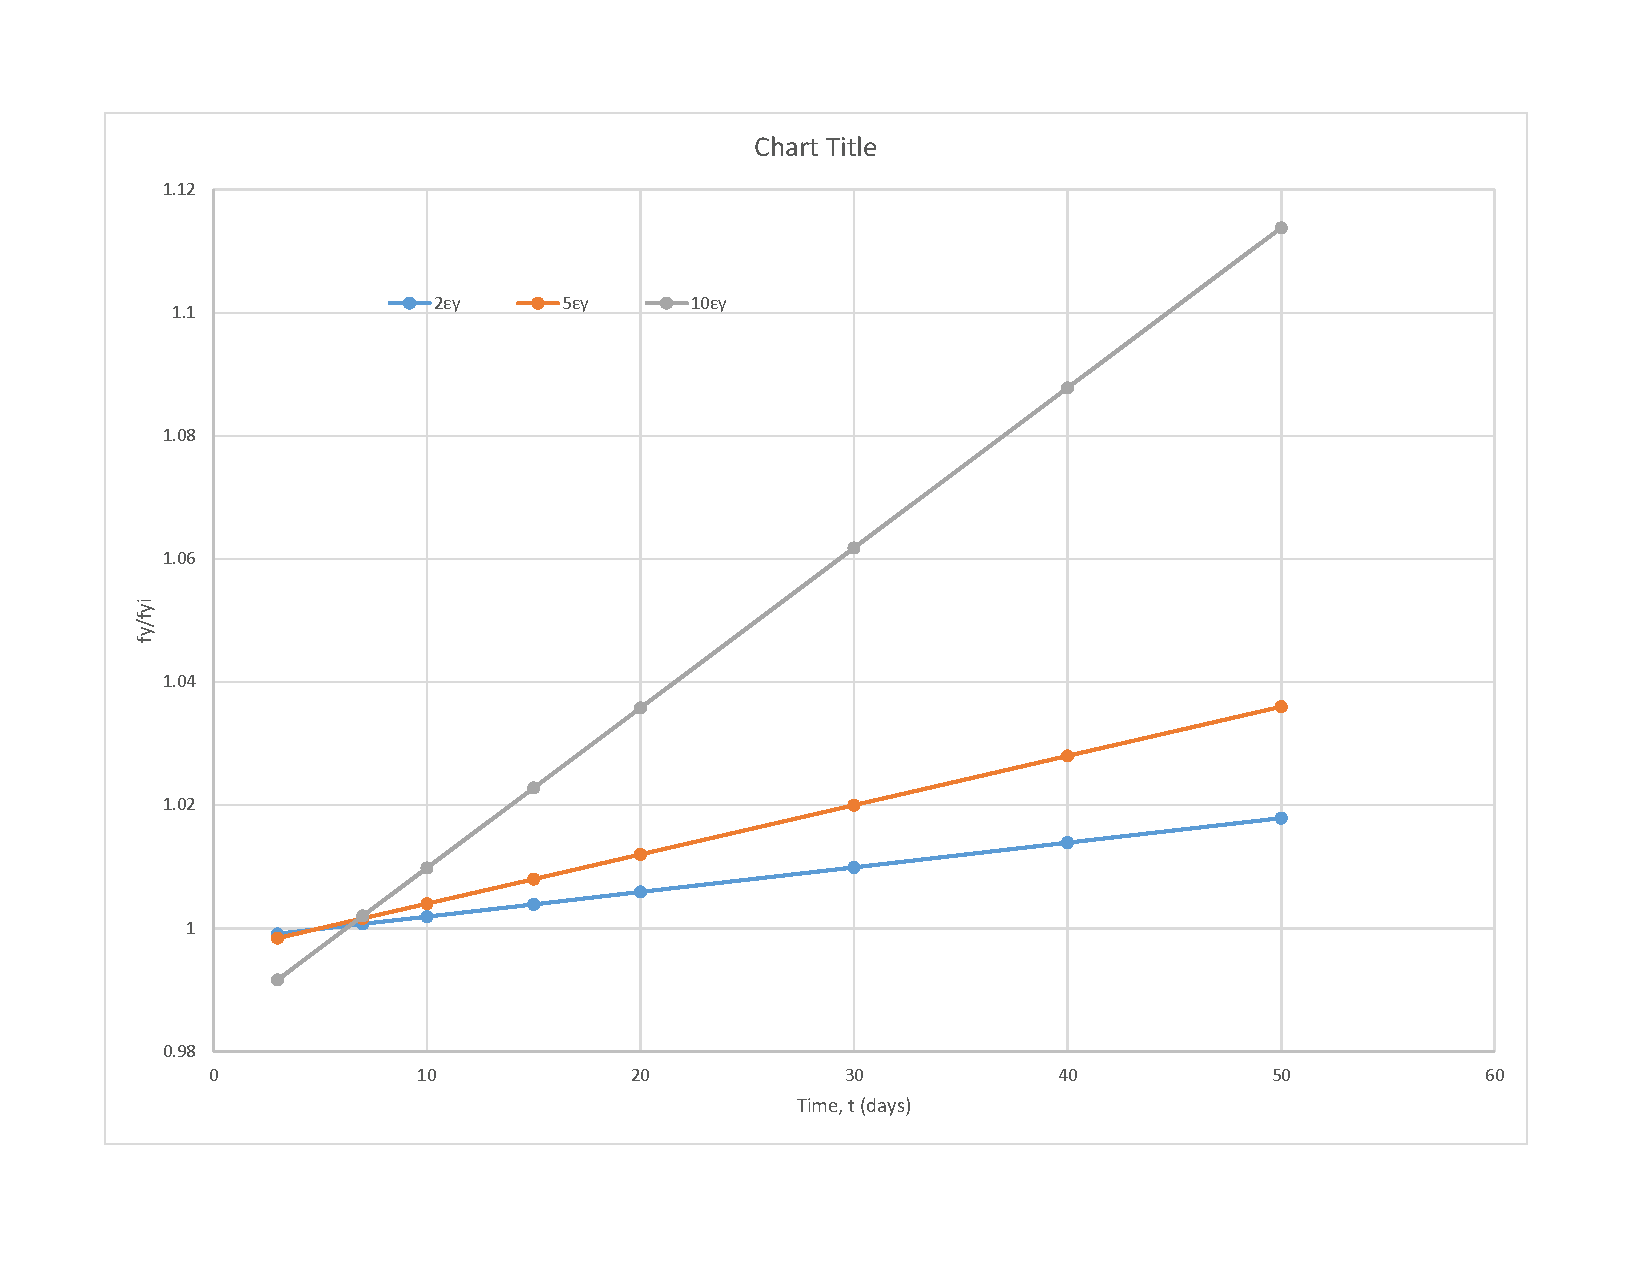
\includegraphics[width=0.9\textwidth]{Chapter-1/figs/StrainAging_TimeDependent}
\caption{Strain Aging effect on Yield Strength vs Time (days)}
\label{fig:hist4}
\end{figure}


For $10\varepsilon_y$

\begin{equation}
  \frac{f_y}{f_{yi}}=0.0026t+0.9838
  \label{eq.twelve}
\end{equation} 

For $5\varepsilon_y$

\begin{equation}
  \frac{f_y}{f_{yi}}=0.0008t+0.996
  \label{eq.thirteen}
\end{equation} 

For $2\varepsilon_y$

\begin{equation}
  \frac{f_y}{f_{yi}}=0.0004t+0.9979
  \label{eq.fourteen}
\end{equation} 

It is proposed to limit the increase in yield strength to the one obtained at 50 days. These equations are plotted in \fref{fig:hist4}

\section{Experimental campaign}

\section{Multiple Seismic Events}

\subsection{Main Shock Series}

\subsection{Main Shock - After Shock Series}

\section{Future Topics}

\begin{itemize}
	\item Concrete Strength Aging
	\item Welding and Fatigue in Steel Structures
	\item Repair Effects
	\item Main Shock - After Shock Series - Repair Series
\end{itemize}
